% Chapter Template

\chapter{Experimental Details} % Main chapter title
\graphicspath{{Pictures/}}
\label{Chapter4} % Change X to a consecutive number; for referencing this chapter elsewhere, use \ref{ChapterX}

\lhead{Chapter 4. \emph{Experimental Details}} % Change X to a consecutive number; this is for the header on each page - perhaps a shortened title

%----------------------------------------------------------------------------------------
%	SECTION 1
%----------------------------------------------------------------------------------------

\section{Introduction}

This section covers the experimental details of the measurements (d,p) and (p,d) transfer reactions on targets of \textsuperscript{116}Cd, \textsuperscript{114}Cd, and \textsuperscript{116}Sn. These measurements were made using the Q3D magnetic spectrometer located at the Maier-Leibnitz Laboratorium (MLL) in Munich. 

%----------------------------------------------------------------------------------------
%	SECTION 2
%----------------------------------------------------------------------------------------

\section{Experimental Procedure}


 ----------------------------------
%	SUBSECTION 1
%-----------------------------------
\subsection{Ion Source}
Proton and deuteron ion beams were produced in a Stern-Gerlach ion source\cite{sterngerlach}. This was operated without using the polarising Stern-Gerlach magnets, as no polarisation was needed for these measurements. This ion source used an electron cyclotron resonance (ECR) positive ion source, combined with a charge exchange cell. The charge exchange cell was required because the acccelerator required injection of negative ions due to the positive charge on the terminal used to produce the accelerating voltage.

The ECR ion source worked by applying a radio-frequency (RF) signal to a gas of the species of atom which was to be used as the beam. This was done in a constant magnetic field, so that the RF frequency matched the natural gyro-frequency of electrons in that magnetic field. This caused resonant acceleration in free electrons in the gas, which ionised the gas by colliding the resonant electrons with the gas atoms. These positive ions were then passed through a caesium jet in a charge exchange cell, which caused them to pick up two electrons and become negative ions.


\subsection{Tandem Accelerator}
The negative ions from the ion source were injected, via a \SI{150}{\kilo\volt} potential, into the MP tandem Van de Graaff accelerator. This accelerated the ions to \SI{15}{\mega\electronvolt} (deuterons) and \SI{22}{\mega\electronvolt} (protons). A central terminal of the accelerator was charged to a high voltage, which could reach approximately \SI{+15}{\mega\volt}\cite{highvoltage}. 

In the accelerator, negative ions were accelerated towards the central terminal by the electrostatic force. The terminal potential was maintained using pelletron chains. These consisted of a chain made of metal pellets connected by insulating nylon, rotating on two pulleys. One pulley was at the terminal, and the other situated by an inductor, which charged the pellets. After being charged, they transported positive charge to the terminal. Negative charge was transported away by the pellets on their return journey. A carbon stripper foil was placed in the central terminal, such that the beam ions lost their electrons upon passing through it. The newly positive beam ions were consequently accelerated away from the terminal with the same voltage. The energy of the beam $E_{\mathrm{beam}}$ was therefore

\begin{equation}
E_{\mathrm{beam}} = (|q_1| + |q_2|)V\mathrm{,}
\end{equation}

where $|q_1|$ and $|q_2|$ are the magnitude of the charges of the beam ions before and after being stripped of electrons, and $V$ is the terminal voltage. In this experiment, hydrogen beams were used so the beam energy was equal to $2V$, since the beam particles had $-1$ charge before and $+1$ charge after passing through the stripper foil. In this experiment, the voltage was held at \SI{7.5}{\mega\volt} for deuterons, \SI{11}{\mega\volt} for protons, and \SI{4.5}{\mega\volt} for elastic scattering measurements.

A diagram of the tandem accelerator is shown in Figure~\ref{tandemDiagram}. The relative positions of the beam line, terminal, and pelletron chains are shown.

\begin{figure}[h]	
\hspace*{-0.5cm}
\begin{center}	
	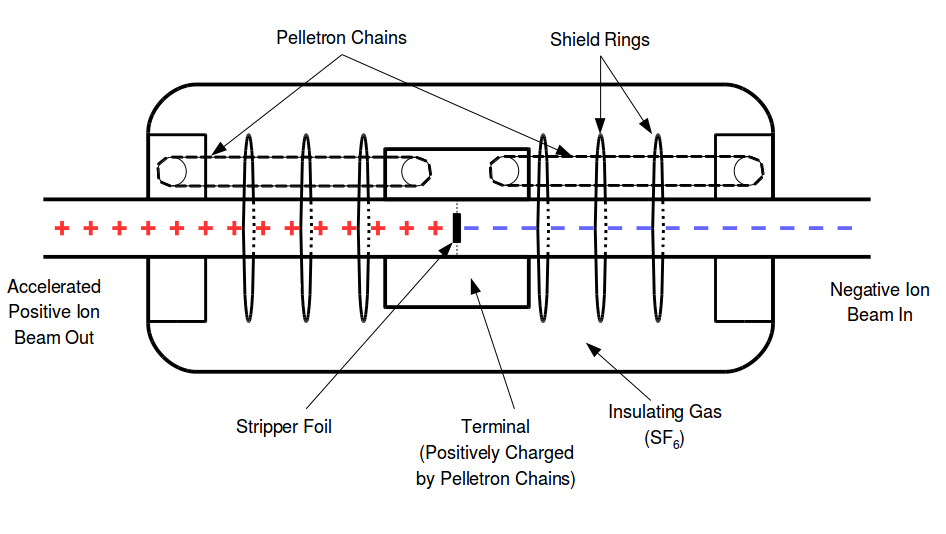
\includegraphics[scale=0.5]{tandem}
\end{center}
			\caption[Schematic of a MP tandem Van de Graaff accelerator]{Schematic of the MP Tandem Van de Graaff generator used at MLL. }
		\label{tandemDiagram}
\end{figure}
\FloatBarrier

\subsection{Beam Delivery}

After acceleration, the beam was then passed through a \SI{90}{\degree} analysing magnet, part of a beam energy calibration system\cite{dollingerfaestermann}. Combining the analysing magnet with analysing slits positioned after the magnets provided a feedback loop, where if the energy was too high or too low, this would be detected and the terminal voltage adjusted accordingly. This system was accurate to one part in $10^4$.

The beam was delivered to the target chamber by a series of quadrupole and dipole magnets to focus and steer respectively.

 ----------------------------------
%	SUBSECTION 2
%-----------------------------------
\subsection{Targets}
The tin targets used in these measurements were oxides, whereas cadmium targets were metallic. The targets were all prepared by evaporating the target material onto a carbon backing with a thickness of 10-\SI{30}{\micro\gram\per\centi\metre\squared}. Each target had a thickness of the order of \SI{100}{\micro\gram\per\centi\metre\squared}. These were mounted on a target ladder, which could hold up to four targets. There were also two more slots on the ladder. One of these was a collimator used for beam tuning, and one was left blank. The target ladders are shown in Figure~\ref{targetLadder}, with targets mounted. Each target could be moved into the path of the beam.

\begin{figure}[h]	
\hspace*{-0.5cm}
\begin{center}	
	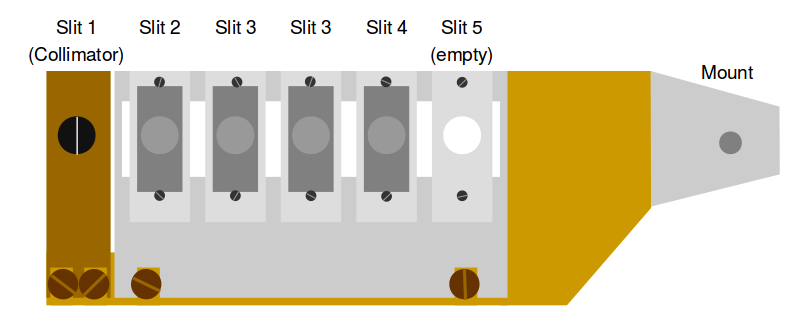
\includegraphics[scale=0.5]{targetladder}
\end{center}
			\caption[Diagram of the MLL target ladder]{Diagram of the target ladder. Slit 5 was empty because the mounting system physically prevented this slot from being moved into the correct position.}
		\label{targetLadder}
\end{figure}
\FloatBarrier

The target ladder was situated in a cylindrical target chamber. The chamber could be isolated from the beamline so it could be vented separately. This allowed the target ladder to be changed. Behind the target, a Faraday cup was positioned. This was connected to a Brookhaven current integrator\cite{bic} to measure the charge collected during each measurement. The spectrograph could be rotated around the target chamber to measure reaction products at different scattering angles. A cartoon of the target chamber is shown in Figure~\ref{targetChamber}, showing the positions of the spectrograph, target ladder, and beam line. At its entrance, there were adjustable slits for the horizontal and vertical collimation. The aperture size was set to \SI{14.03}{\milli\steradian}, except for at forward scattering angles, where it was set to \SI{7.25}{\milli\steradian}. This was done to prevent detector saturation due to large elastic scattering cross sections at these angles.

\begin{figure}[h]	
\hspace*{-0.5cm}
\begin{center}	
	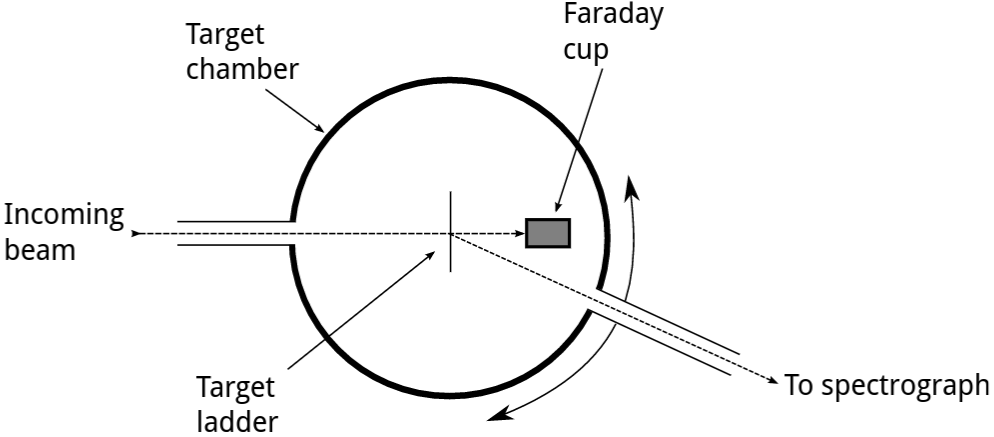
\includegraphics[scale=0.3]{targetchamber}
\end{center}
			\caption[Schematic of the Q3D target chamber]{A cartoon of the target chamber\cite{stuart}. Note that a faraday cup is placed behind the target to measure the beam current, and that the angle of the spectrograph can be altered.}
		\label{targetChamber}
\end{figure}
\FloatBarrier

 ----------------------------------
%	SUBSECTION 3
%-----------------------------------

\subsection{The Q3D Spectrograph}

The Q3D spectrograph separated ejectiles dispersively by their momentum. The position was measured to determine the momentum and excitation. A magnetic field was used to separate the ejectiles by applying a radial field.

Comparing the condition for circular motion

\begin{equation}
	F = \frac{mv^2}{\rho}\mathrm{,}
\end{equation}

where $F$ is the radial force experienced by the reaction product, $m$ is the mass of the reaction product, $v$ is the velocity, and $\rho$ is the radius of curvature, with the Lorentz equation for a charged particle moving perpendicular to a magnetic field,

\begin{equation}
	F = qBv\mathrm{,}
\end{equation}

where $F$ is the magnitude of the force, $q$ is the charge, $B$ is the magnetic field strength and $v$ is the velocity, gives 

\begin{equation}
	mv = qB\rho\mathrm{.}
\end{equation}

It can be seen that that the radius of curvature depends linearly on the momentum. This shows how the Q3D spectrometer separated ejectiles radially in the experiment.

The spectrograph did this with one quadrupole magnet and three dipole magnets. Figure~\ref{Q3D} is a cartoon of the spectrograph, showing the configuration of the magnets. It can be seen that the dipole magnets provided the radial bending.
 
\begin{figure}[h]	
\hspace*{-0.5cm}
\begin{center}	
	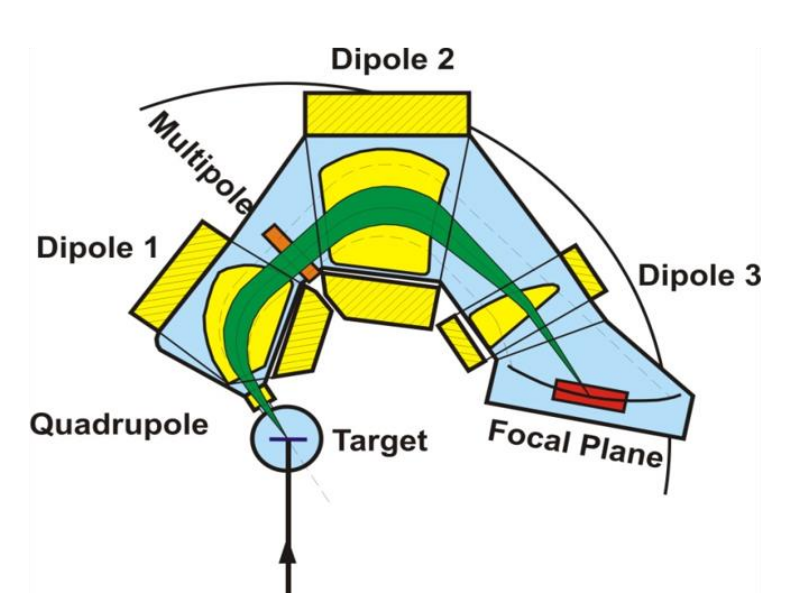
\includegraphics[scale=0.4]{benq3d}
\end{center}
			\caption[Schematic diagram of the Q3D magnetic spectrograph]{Sketch of the Q3D spectrograph, showing paths of ejectiles from the target to the focal plane.~\cite{dollingerfaestermann}}
		\label{Q3D}
\end{figure}
\FloatBarrier

While the dipole magnets provided the radial bending, the quadrupole increased the vertical acceptance of the spectrometer by focusing ejectiles into the focal plane of the detector. There was also a multipole element to correct for kinematic broadening~\cite{scheerer}. Overall, the ejectiles were vertically focused and bent horizontally into this focal plane, where a detector was placed.

 ----------------------------------
%	SUBSECTION 4
%-----------------------------------
\subsection{Focal Plane Detectors}

A detector system was placed along the focal plane to measure the position of the ejectiles, and therefore their momentum. Furthermore, the species of interest could be identified via the amount of energy lost in different parts of the detector system. 

There were three separate detectors in the focal plane detector system. Two were Multi-Wire Proportional Counters (MWPCs) and one was a plastic scintillator. The layout of the detectors is shown in Figure~\ref{detectorSketch}, with the MWPCs shown in front of the scintillator.

\begin{figure}[h]	
\hspace*{-0.5cm}
\begin{center}	
	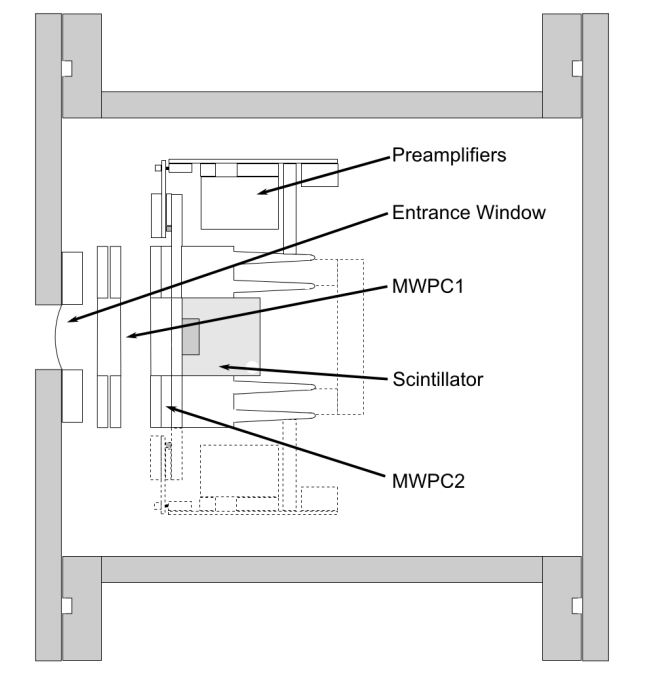
\includegraphics[scale=0.5]{focalplanesketch}
\end{center}
			\caption[Diagram of the focal plane detector]{Diagram of the layout of the focal plane detector~\cite{gillespie,mllreport}. The reaction products enter from the left, then pass through the two MWPCs and come to rest in the scintillator.}
		\label{detectorSketch}
\end{figure}
\FloatBarrier

An MWPC comprises a sandwich-like setup of parallel wires surrounded by isobutane gas, between two cathode foils. Upon being struck by a particle, the gas ionises. In regions of higher field near to the anode, this creates an avalanche. The electrons gather on an anode wire, while the ions gather on the cathode. The total signal from the anodes is proportional to the energy deposited by the incoming particle.

On the second of the MWPCs at the Munich Q3D, the cathode foil was split into multiple strips, where the charge accumulated on each could be measured. This allowed the position of the ionisation of the gas along the focal plane to be measured, and with it the position of the impact of the reaction product.

An event consisted of 3-6 adjacent strips registering a signal. The position was determined by fitting the collected charge on these strips with a Gaussian function. This process of determining the position is illustrated in Figure~\ref{posCathode}. Note that the cathode strips were equally spaced along the focal plane.

\begin{figure}[h]	
\hspace*{-0.5cm}
\begin{center}	
	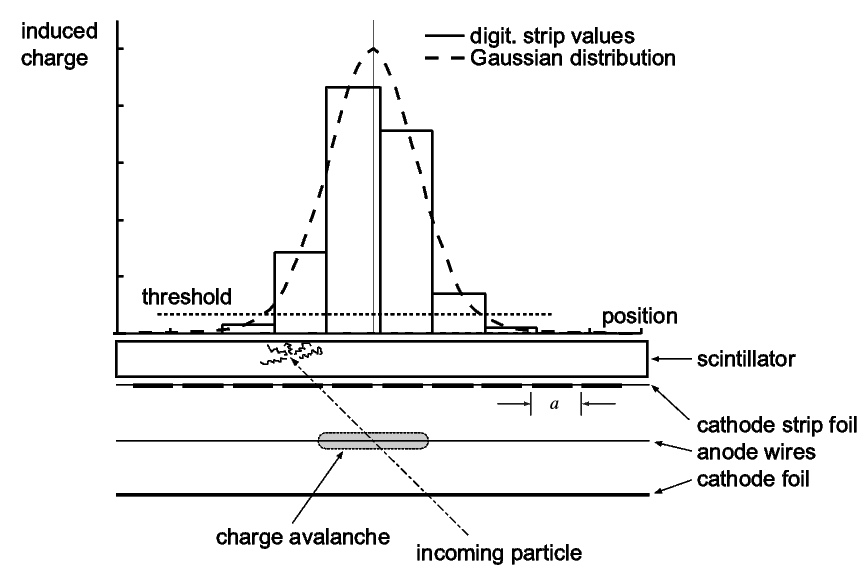
\includegraphics[scale=0.4]{cathodestrip}
\end{center}
			\caption[Illustration of the priciple of cathode strip detectors]{Illustration of the principle of the cathode strip method of focal plane position determination~\cite{mllreport}. $a$ is the repetition distance between cathode strips. A Gaussian distribution was fit to all of the cathode signals which exceed the threshold. }
		\label{posCathode}
\end{figure}
\FloatBarrier

Behind the two MWPCs, a plastic scintillator was placed to absorb the rest of the energy of an incoming reaction product. A scintillation detector works by converting the energy of an incoming particle into light, where the number of photons is proportional to the energy deposited by the particle. This light strikes a photocathode, which emits electrons via the photoelectric effect. The electrons are then multiplied in a photomultiplier tube, so the current is proportional to the energy deposited by the original incoming particle. This is then passed through a resistor, so the voltage across the resistor is then proportional to the energy of the initial reaction product.

The change in energy $\Delta E$ through both MWPCs was proportional to the anode signals. The corresponding final energy $E$ could be measured by the scintillator. Particles from the the reactions of interest could be identified through a comparison of the signals from the MWPCs and the scintillator.


\section{Experimental Considerations}

\subsection{Momentum Matching}

For \textsuperscript{116}Cd, \textsuperscript{114}Cd, and \textsuperscript{116}Sn, the states populated were in between the $N = 50, 82$ shell closures. This region corresponds to the $3s, 2d, 1h_{11/2}, \mathrm{and }1g_{7/2}$ orbitals. Some population of the states above and below may also be expected.

The (p,d) and (d,p) reactions favour population of states with low angular momentum.

The Q value of a reaction is the difference in rest mass energies of the initial and final states\cite{krane}. The deuteron is weakly bound, so the $Q$ value for these reactions are low. In contrast, the alpha particle is very strongly bound\cite{krane}, so transfer reactions involving alpha particles have high $Q$ values.

For a two body reaction with a moving projectile, and both target and recoil nuclei being stationary,

\begin{equation}
Q =\frac{p_i^2}{2m_i} - \frac{p_f^2}{2m_f}\mathrm{,}
\end{equation}

where $p_i$ and $m_i$ are the linear momentum and mass of the projectile, and $p_f$ and $m_f$ are the linear momentum and mass of the ejectile. The magnitude of the momentum transfer is 

\begin{equation}
q = |{\bf p}_i - {\bf p}_f|\mathrm{,}
\end{equation}

which depends on $Q$.

This linear momentum transfer affects the angular momentum transfer. Consider the classical expression for angular momentum

\begin{equation}
{\bf L} = {\bf r} \times {\bf p}\mathrm{,}
\end{equation}

where linear momentum is ${\bf p}$, and position relative to the centre of rotation is ${\bf r}$. In a direct reaction, ${\bf r}$ is approximately ${\bf R}$, the nuclear radius. Multiple step reactions are more likely if the projectile passes through the centre of the nucleus. Further away from the nucleus than the nuclear radius, any reaction becomes unlikely.

In this semiclassical approach, the angular momentum transfer increases with higher linear momentum transfer, and this increases with $Q$. For the reactions of interest, which have low $Q$ values, the population of states of low angular momentum was favoured.

\subsection{Angle and Energy Selection}


This semiclassical picture can also help with understanding how the angular distribution is affected by the angular momentum transfer $\delta {\bf l}$ and the beam energy $E_{\mathrm{lab}}$. The angular momentum transfer is

\begin{equation}
\Delta {\boldsymbol \ell} = {\bf R} \times {\bf q}\mathrm{,}
\end{equation}

so the maximum amount of transferred angular momentum is

\begin{equation}
\Delta \ell = R q \mathrm{.}
\end{equation}

Also,

\begin{equation} \label{momentumTransfer}
q = \sqrt{p_i^2 + p_f^2 - 2 p_i p_f \cos \theta}\mathrm{,}
\end{equation}

where $\theta$ is the scattering angle. With the knowledge that $R$ is constant, and that $p_i^2$ and $p_f^2$ are small due to the low $Q$ value of this reaction, it can be seen that $\delta l$ can be increased by increasing the scattering angle.

Conversely, the scattering angle can be reduced by increasing $E_{lab}$. For a given $q$, if the lab energy (and therefore projectile momentum) increases, the scattering angle becomes smaller. This is because the cross term in Equation~\ref{momentumTransfer} becomes large with a smaller scattering angle if $p_i$ and $p_f$ are larger. This means that angular distributions for all of the possible populated states become forward peaked at high energies.

This angle and energy dependence of $\delta l$ persist in a more rigorous DWBA model of the reaction, as shown in Figure~\ref{energyDists}. It is clear that a larger $\delta l$ results in a peak in cross-section at larger angles, increasing $E_{lab}$ makes the angular distributions more forward peaked, and that in general, low $\delta l$ is favoured. It is also shown that the cross sections for transfer reactions become much lower at smaller energies. This is because the projectiles are less likely to overcome the Coulomb barrier at lower energies.

\begin{figure}[h]	
\hspace*{-0.5cm}
\begin{center}
	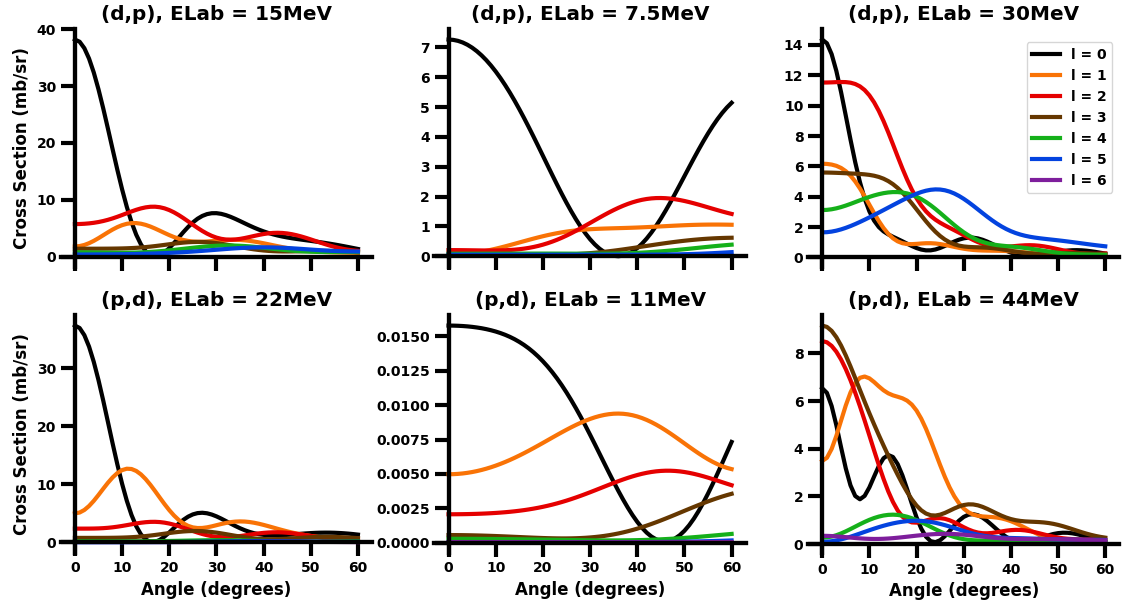
\includegraphics[width=\textwidth]{energydist}
\end{center}
			\caption[Angular distributions for (p,d) and (d,p) at different lab energies]{Angular distributions for (p,d) and (d,p) reactions on \textsuperscript{116}Cd. These are to a hypothetical ground state in the daughter nucleus.}
		\label{energyDists}
\end{figure}
\FloatBarrier

These effects were considered when selecting the angles and energies to measure at. \SI{22}{\mega\electronvolt} was chosen for all (p,d) reactions and \SI{15}{\mega\electronvolt} was chosen for (d,p). This was such that the peaks of different angular momentum states were distinct, and the cross-sections were sufficiently high. The angles where the $\ell = 0,2,4,5$ distributions peaked were chosen for the measuring angles. These were $\theta = (10, 18, 31, 40)^\mathrm{o}$ for (d,p), and $\theta = (8, 17, 31, 39)^\mathrm{o}$ for (p,d) An additional angle which lay at the peak of the $l = 3$ distribution ($\theta = 25^\mathrm{o}$ for (d,p), $\theta = 26^\mathrm{o}$ for (p,d)) was also measured with a smaller amount of beam time to distinguish between $\ell = 1$ and $\ell = 3$ states. The additional angle also ameliorated the obscuring effect of contaminants.

\subsection{Target Thickness} \label{ssec:tthick}

The thickness of the targets were an important consideration, because to calculate a cross-section, the number of particles that the beam may interact with must be known.

The target thickness was calculated by performing a reaction with a known cross-section, and deducing the target thickness from the yield collected for this reaction. The reaction used was elastic scattering, with the Rutherford cross-section used to calculate the cross-sections.

Rutherford scattering is the scattering of charged particles by the Coulomb field. The differential cross-section for Rutherford scattering in \si{\milli\barn\per\steradian}   is given by
\begin{equation}
\frac{\mathrm{d}\sigma}{\mathrm{d}\Omega}= 1.296\bigg(\frac{Z_bZ_t}{E_{\mathrm{lab}}}\bigg)^2\frac{1}{\sin^4\frac{\theta}{2}}
\end{equation}

where $Z_b$ and $Z_t$ are the proton numbers of the beam and target respectively, $E_{\mathrm{lab}}$ is the beam energy, and $\theta$ is the scattering angle\cite{rutherford,rutherfordformula}.

A beam energy and angle were selected such that the Rutherford cross-section was a valid approximation of the actual cross-section. This was best done at low energies so that the projectiles were less likely to get too close to the nucleus to assume pure Coulomb scattering. The chosen scattering angle could not be small because of the large scattering cross-section at these angles, which would swamp the detector. For \SI{9}{\mega\electronvolt} deuterons at a \SI{20}{\degree} scattering angle, which was the configuration used for target thickness measurements, it can be seen in Fig~\ref{elasticsRatio} that the elastic scattering cross section differed by 2\% from the Rutherford cross section.

\begin{figure}[h]	
\hspace*{-0.5cm}
\begin{center}
	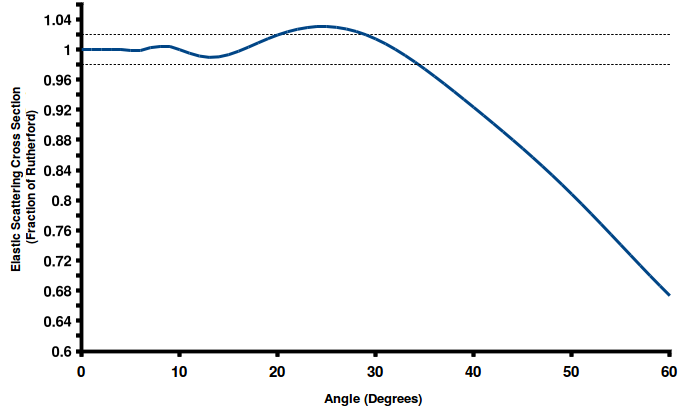
\includegraphics[width=\textwidth]{elasticsratio}
\end{center}
			\caption[Fraction of Rutherford cross-section for 9 MeV deuteron elastic scattering]{Fraction of Rutherford cross-section for 9 MeV deuteron elastic scattering. The dotted lines mark where the deviation from the Rutherford cross-section is 2\%. At 20 degrees, the deviation is approximately 2\%.}
		\label{elasticsRatio}
\end{figure}
\FloatBarrier


\subsection{Contaminants}

The targets were carbon-backed and some targets were oxides. Targets can also become oxidised with exposure to air. The targets also had varying isotopic purity.

The effect of light mass contaminants is the presence of large, broad peaks in the spectra. They are large because the states populated from reactions on \textsuperscript{16}O and \textsuperscript{12}C had large cross-sections from the reaction. The peaks were broad because they were out of focus, as the field was set to focus the ejectiles for reactions on the targets of interests which had a smaller kinematic shift. An example of a light-mass contaminant peak is shown in Fig~\ref{lmContaminant}.

\begin{figure}[h]	
\hspace*{-0.5cm}
\begin{center}
	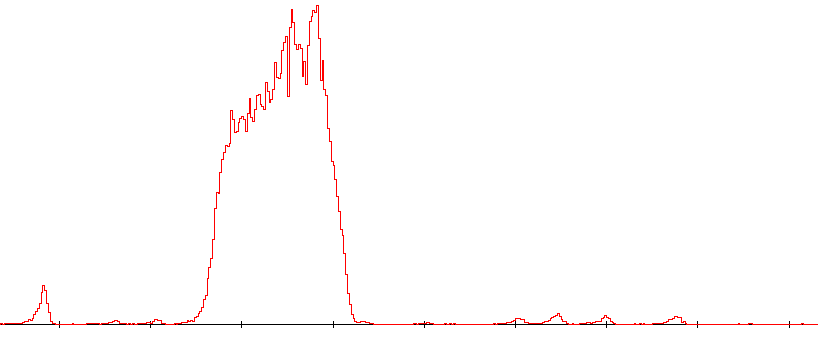
\includegraphics[width=\textwidth]{lmContaminant}
\end{center}
			\caption[Example of a light mass contaminant peak]{Example of a light mass contaminant peak. This is in the \textsuperscript{116}Sn (d,p) spectrum at a \SI{30}{\degree} scattering angle. The contaminant peak obscures states at approximately \SI{2.5}{\mega\electronvolt}. This is the \textsuperscript{12}C(d,p)\textsuperscript{13}C reaction, where the \textsuperscript{13}C is in its ground state.}
		\label{lmContaminant}
\end{figure}
\FloatBarrier

These light-mass contaminant peaks moved along the focal plane at different angle measurements. This meant that no state was obscured by the contaminant at every angle, but conversely it meant that more states were affected overall. The obscuring effect of the contaminant peaks was ameliorated by taking the bonus additional measurement.

As well as light mass contaminants, isotopic contaminants were present in the targets, because the enriching process did not fully erase the presence of other natural isotopes. Because each significant isotopic contaminant is at approximately 1\% enrichment, strong isotopic contaminant peaks appear with approximately 1\% of the yield of strong peaks for the desired reaction. This means they were visible, but at the limit of what could be seen, with less than 100 counts in the peaks. They were identifiable by a $qB\rho$ calibration of the spectra.

\subsection{Magnetic Field Settings}

The nuclear states were probed up to approximately \SI{4}{\mega\electronvolt}. This was not possible with one magnetic field setting of the Q3D, because the Q3D spectrometer had a large dispersion. This meant that states of different energy were separated more along the focal plane, and in this case so much that the 0-\SI{4}{\mega\electronvolt} range was not covered by the focal plane detector. In fact, the energy range covered by one measurement was approximately \SI{1}{MeV}.

This meant that multiple magnetic field settings had to be made. For (d,p), three field settings were used for each target at each angle, while for (p,d), four were used. It was ensured that there was an overlap of states between these measurements to allow for an accurate energy calibration.